\documentclass[11pt,a4paper]{article}
\usepackage[margin=1in]{geometry}
\usepackage{graphicx}
\usepackage{booktabs}
\usepackage{hyperref}
\usepackage{amsmath}
\usepackage{float}
\usepackage{caption}
\usepackage{multirow}
\usepackage{xcolor}
\usepackage{siunitx}
\usepackage{tabularx}

\title{Robustness of 3D U-Net Dose Prediction to\\Clinically Plausible CT Perturbations}
\author{OpenKBP Project}
\date{February 24, 2026}

\begin{document}

\maketitle

\begin{abstract}
We evaluate the robustness of a 3D U-Net dose prediction model to five families of clinically plausible CT perturbations: acquisition noise, HU calibration shift, low-frequency bias field, resolution degradation, and dental metal artifacts. Unlike adversarial attacks that exploit worst-case gradient directions, these perturbations model realistic imaging variability encountered in radiotherapy workflows. Evaluated on 40 head-and-neck cancer patients at up to five severity levels per perturbation, the model demonstrates remarkable stability: four of five perturbation families cause less than 1.5\% DVH degradation even at extreme amplitudes. Only resolution degradation produces substantial impact, with DVH degradation beginning at the mildest level (+1.5\% at L0) and reaching +18.2\% at L4. Bone-weighted calibration shift shows a late take-off at L5 (+11.2\% DVH). These finer-grained severity sweeps identify specific threshold amplitudes for each perturbation, supporting targeted quality control recommendations for clinical deployment.
\end{abstract}

\tableofcontents
\newpage

\section{Introduction}

\subsection{Clinical Motivation}

CT imaging serves as the foundation of radiotherapy treatment planning. In clinical practice, CT images vary due to scanner hardware differences, acquisition protocols, reconstruction parameters, patient-specific artifacts (e.g., dental implants), and normal quantum noise. A dose prediction model deployed across clinical sites must produce stable predictions despite this inherent imaging variability.

\subsection{Relationship to Adversarial Evaluation}

A companion report (Report~1) evaluates the same model under adversarial attacks (FGSM, PGD) that exploit worst-case gradient directions to maximally degrade predictions. Those attacks revealed 21--30\% dose score degradation at $\epsilon = 0.01$ ($\approx$41~HU). This report takes a complementary approach: instead of worst-case perturbations, we apply \emph{physically motivated} perturbations that model realistic CT imaging variability. This distinction is critical for clinical deployment---adversarial robustness measures theoretical vulnerability, while perturbation robustness measures practical reliability.

\subsection{Model Overview}

The evaluated model is a 3D U-Net with Squeeze-and-Excitation (SE) blocks, trained on the OpenKBP dataset for head-and-neck radiotherapy dose prediction:
\begin{itemize}
    \item \textbf{Architecture}: 3D U-Net, 6 encoder / 5 decoder stages (64--512 filters), SE blocks on deep layers, InstanceNorm, residual connections
    \item \textbf{Input}: CT volume (128$^3$) + 10 structure masks
    \item \textbf{Output}: Predicted dose distribution (128$^3$)
    \item \textbf{Training}: Masked MAE loss, PTV weighting (4.0$\times$), data augmentation, mixed precision
    \item \textbf{Baseline performance}: DVH Score 2.535, Dose Score 3.731~Gy
\end{itemize}

\section{Methods}

\subsection{Perturbation Families}

We define five perturbation families spanning the major sources of CT imaging variability in radiotherapy. Each family is tested at multiple severity levels to identify degradation thresholds. P1--P3 and P5 use levels L1--L5 (mild to extreme); P4 (resolution) uses L0--L4 since degradation begins at the mildest settings. Table~\ref{tab:perturbations} summarizes all perturbations and their parameters.

\begin{table}[H]
\centering
\caption{CT perturbation families with parameters at each severity level. All values in HU (Hounsfield Units) or voxels as indicated. L0 is only used for P4; L5 is not used for P4.}
\label{tab:perturbations}
\small
\begin{tabularx}{\textwidth}{@{}l l X@{}}
\toprule
\textbf{Perturbation} & \textbf{Physical Model} & \textbf{Levels (key parameters)} \\
\midrule
P1: Acq.\ Noise & Heteroscedastic Gaussian & L1: $\sigma_\text{soft/bone}{=}8/12$; L2: 15/25; L3: 30/50; L4: 60/100; L5: 100/160\,HU \\[4pt]
P2: Bone Shift & HU calibration error & L1: $\Delta_\text{soft/bone}{=}5/50$; L2: 10/100; L3: 25/250; L4: 50/500; L5: 100/1000\,HU \\[4pt]
P3: Bias Field & Low-freq.\ cosine harmonics & L1: 10; L2: 20; L3: 50; L4: 100; L5: 200\,HU amplitude \\[4pt]
P4: Resolution & Anisotropic Gaussian blur & L0: $\sigma_{z/xy}{=}0.5/0.25$; L1: 1.0/0.5; L2: 2.0/1.0; L3: 3.0/1.5; L4: 4.0/2.0\,vox \\[4pt]
P5: Dental Art. & Radial streak pattern & L1: 150\,HU/8 streaks; L2: 300/12; L3: 500/16; L4: 800/20; L5: 1200/24 \\
\bottomrule
\end{tabularx}
\end{table}

\subsubsection{P1: Acquisition Noise}

Models heteroscedastic quantum noise with tissue-dependent variance. The noise standard deviation is higher in bone ($\sigma_\text{bone}$) than in soft tissue ($\sigma_\text{soft}$), reflecting the physics of photon attenuation:
\begin{equation}
\text{CT}_\text{perturbed} = \text{CT} + \mathcal{N}(0, \sigma(x)^2), \quad \sigma(x) = \begin{cases} \sigma_\text{bone} & \text{if CT}(x) > 1500 \\ \sigma_\text{soft} & \text{otherwise} \end{cases}
\end{equation}
where 1500 corresponds to the cortical bone threshold in OpenKBP coordinates ($\approx$476 standard HU). At L1, noise magnitudes (8--12~HU) are within typical CT scanner noise ranges (10--50~HU); at L2, the 25~HU bone noise represents a noisier acquisition.

\subsubsection{P2: Bone-Weighted HU Calibration Shift}

Simulates systematic HU calibration drift that affects bone and soft tissue differently, as occurs with CT tube aging or cross-scanner variation. A sigmoid function provides smooth blending:
\begin{equation}
\Delta(x) = s \cdot \left[\Delta_\text{soft} + (\Delta_\text{bone} - \Delta_\text{soft}) \cdot \frac{1}{1 + e^{-(\text{CT}(x)-1500)/200}}\right], \quad s \sim \text{Uniform}\{-1, +1\}
\end{equation}
The random sign $s$ models bidirectional calibration error. The sigmoid transition (center 1500, width 200) prevents discontinuities at tissue boundaries.

\subsubsection{P3: Low-Frequency Bias Field}

Models spatially smooth intensity variations from RF non-uniformity or scatter:
\begin{equation}
B(x,y,z) = A \cdot \frac{\sum_{k=1}^{K} w_k \prod_{d \in \{x,y,z\}} \cos(2\pi f_{k,d} \cdot d + \phi_{k,d})}{\max|B|}
\end{equation}
where $K=3$ harmonics with random frequencies $f \in [0.5, 2.5]$ cycles per FOV, phases $\phi \in [0, 2\pi)$, and weights $w \in [0.3, 1.0]$. The amplitude $A$ controls the maximum HU deviation.

\subsubsection{P4: Resolution Degradation}

Models reduced spatial resolution from thicker CT slices or smoother reconstruction kernels via anisotropic Gaussian blurring:
\begin{equation}
\text{CT}_\text{perturbed} = \text{CT} * G(\sigma_z, \sigma_{xy}, \sigma_{xy})
\end{equation}
where $G$ is a 3D Gaussian kernel applied with \texttt{scipy.ndimage.gaussian\_filter}. The z-axis receives stronger blur than the xy-plane, reflecting the typical anisotropy of CT acquisitions where slice spacing exceeds in-plane resolution.

\subsubsection{P5: Dental Metal Artifact}

Simulates streak artifacts from dental implants anchored to the mandible centroid. The artifact consists of radial streaks in the axial plane with exponential radial decay and Gaussian z-spread:
\begin{equation}
\text{streak}(\theta) = \sum_{i=1}^{N} (-1)^i \exp\!\left(-\frac{(\theta - \theta_i)^2}{2w^2}\right), \quad w = \frac{\pi}{1.5N}
\end{equation}
where $N$ is the number of streaks and $\theta_i$ are random angles. The streak pattern is modulated by radial decay $e^{-r/40}$ and z-axis Gaussian decay ($\sigma_z = 3$ slices). A high-HU metal spot (3000--3500~HU) is placed at the mandible centroid within a 3-voxel radius.

\subsection{Experimental Setup}

\begin{itemize}
    \item \textbf{Dataset}: 40 validation patients (pt\_201--pt\_240) from the OpenKBP dataset
    \item \textbf{Conditions}: 27 total (1 baseline + 5 perturbations $\times$ 4--5 levels each)
    \item \textbf{Seeding}: Deterministic (seed 42) for reproducibility; perturbation randomness is per-patient
    \item \textbf{CT normalization}: [0, 4095] $\rightarrow$ [0, 1] (12-bit range per OpenKBP specification)
    \item \textbf{Perturbation domain}: Applied in raw HU space before normalization
    \item \textbf{Hardware}: NVIDIA RTX 3090 GPU (RunPod), TensorFlow 2.18.0
\end{itemize}

\subsection{Evaluation Metrics}

\begin{itemize}
    \item \textbf{Dose Score}: Voxel-wise MAE (Gy) within the \texttt{possible\_dose\_mask} region
    \item \textbf{DVH Score}: Mean absolute error of DVH statistics ($D_{0.1\text{cc}}$, mean dose for OARs; $D_1$, $D_{95}$, $D_{99}$ for PTVs) across all structures
    \item \textbf{Delta}: Absolute and percentage change from baseline for both metrics
\end{itemize}

Evaluation uses the OpenKBP \texttt{DoseEvaluator} class with unnormalized (Gy) dose values for both reference and prediction.

\section{Results}

\subsection{Summary}

Table~\ref{tab:results} presents the complete results across all 27 conditions. The model achieves baseline performance of 3.731~Gy dose score and 2.535 DVH score.

\begin{table}[H]
\centering
\caption{Dose and DVH scores across all perturbation conditions. $\Delta$ columns show change from baseline. Bold values indicate degradation $>$5\%.}
\label{tab:results}
\small
\begin{tabular}{@{}lS[table-format=1.3]S[table-format=1.3]S[table-format=+2.1]S[table-format=+2.1]@{}}
\toprule
\textbf{Condition} & {\textbf{Dose (Gy)}} & {\textbf{DVH}} & {$\boldsymbol{\Delta}$\textbf{Dose (\%)}} & {$\boldsymbol{\Delta}$\textbf{DVH (\%)}} \\
\midrule
Baseline & 3.731 & 2.535 & {---} & {---} \\
\midrule
P1\_noise / L1 & 3.731 & 2.535 & +0.0 & +0.0 \\
P1\_noise / L2 & 3.733 & 2.538 & +0.1 & +0.1 \\
P1\_noise / L3 & 3.737 & 2.543 & +0.2 & +0.3 \\
P1\_noise / L4 & 3.742 & 2.559 & +0.3 & +1.0 \\
P1\_noise / L5 & 3.742 & 2.571 & +0.3 & +1.4 \\
\midrule
P2\_bone\_shift / L1 & 3.730 & 2.531 & -0.0 & -0.1 \\
P2\_bone\_shift / L2 & 3.740 & 2.544 & +0.3 & +0.4 \\
P2\_bone\_shift / L3 & 3.751 & 2.519 & +0.5 & -0.6 \\
P2\_bone\_shift / L4 & 3.793 & 2.572 & +1.7 & +1.5 \\
P2\_bone\_shift / L5 & 3.916 & 2.818 & \bfseries +5.0 & \bfseries +11.2 \\
\midrule
P3\_bias\_field / L1 & 3.732 & 2.535 & +0.0 & +0.0 \\
P3\_bias\_field / L2 & 3.730 & 2.534 & -0.0 & -0.0 \\
P3\_bias\_field / L3 & 3.736 & 2.534 & +0.2 & -0.0 \\
P3\_bias\_field / L4 & 3.733 & 2.524 & +0.1 & -0.4 \\
P3\_bias\_field / L5 & 3.759 & 2.545 & +0.8 & +0.4 \\
\midrule
P4\_resolution / L0 & 3.739 & 2.573 & +0.2 & +1.5 \\
P4\_resolution / L1 & 3.780 & 2.636 & +1.3 & +4.0 \\
P4\_resolution / L2 & 3.885 & 2.729 & +4.1 & \bfseries +7.7 \\
P4\_resolution / L3 & 3.982 & 2.824 & \bfseries +6.7 & \bfseries +11.4 \\
P4\_resolution / L4 & 4.124 & 2.995 & \bfseries +10.5 & \bfseries +18.2 \\
\midrule
P5\_dental / L1 & 3.729 & 2.541 & -0.0 & +0.3 \\
P5\_dental / L2 & 3.730 & 2.545 & -0.0 & +0.4 \\
P5\_dental / L3 & 3.730 & 2.552 & -0.0 & +0.7 \\
P5\_dental / L4 & 3.731 & 2.557 & +0.0 & +0.9 \\
P5\_dental / L5 & 3.732 & 2.555 & +0.0 & +0.8 \\
\bottomrule
\end{tabular}
\end{table}

\subsection{Score Degradation Overview}

Figure~\ref{fig:summary_bars} shows the dose and DVH score degradation across all conditions. Resolution degradation (P4) is visually dominant; all other perturbations are near-zero.

\begin{figure}[H]
\centering
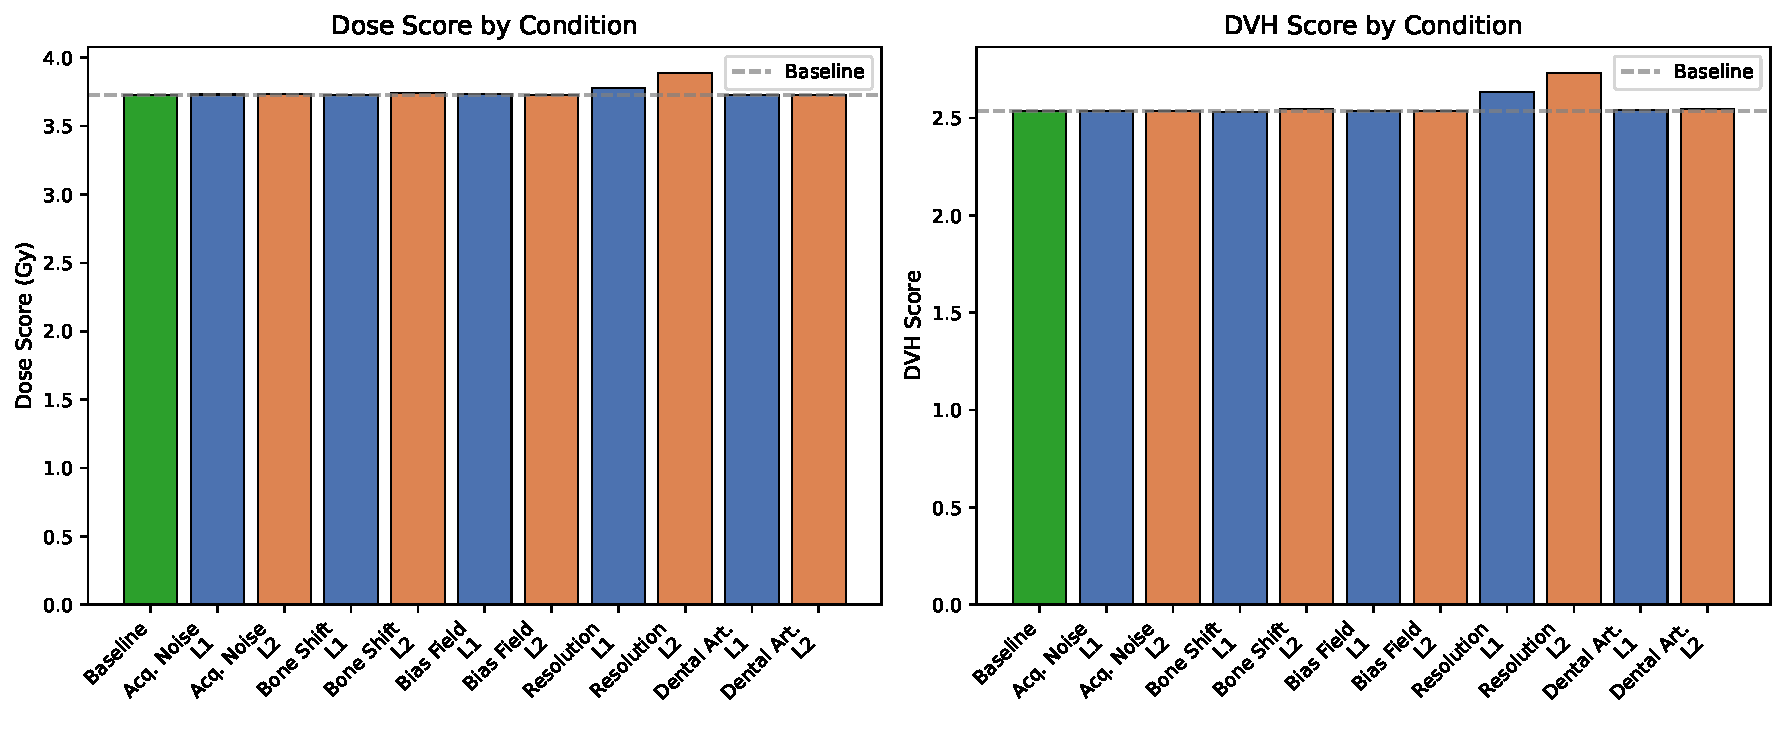
\includegraphics[width=0.95\textwidth]{figures/summary_bars.pdf}
\caption{Dose score (left) and DVH score (right) across all perturbation conditions. P4 (resolution degradation) is the only perturbation producing visible degradation.}
\label{fig:summary_bars}
\end{figure}

\subsection{Degradation Curves}

Figure~\ref{fig:curves} plots dose and DVH score as a function of perturbation severity for each perturbation family. The finer-grained severity sweep (up to 5 levels per perturbation) reveals distinct take-off behaviors:
\begin{itemize}
    \item \textbf{P4 (Resolution)}: Continuous, approximately linear degradation beginning at the mildest level (L0: +1.5\% DVH) and reaching +18.2\% DVH at L4. There is no threshold below which the model is invariant to spatial blur---even half-voxel Gaussian smoothing produces measurable impact.
    \item \textbf{P2 (Bone Shift)}: Flat through L3 ($\Delta_\text{bone} \leq 250$~HU), then takes off at L4 (+1.5\% DVH) with a sharp jump to L5 (+11.2\% DVH, $\Delta_\text{bone} = 1000$~HU). This late, sudden onset indicates a threshold effect near $\Delta_\text{bone} \approx 500$~HU.
    \item \textbf{P1 (Noise), P3 (Bias Field), P5 (Dental)}: All three remain essentially flat through their highest levels ($\leq$1.4\% DVH), confirming robust invariance to even extreme intensity-domain perturbations.
\end{itemize}

\begin{figure}[H]
\centering
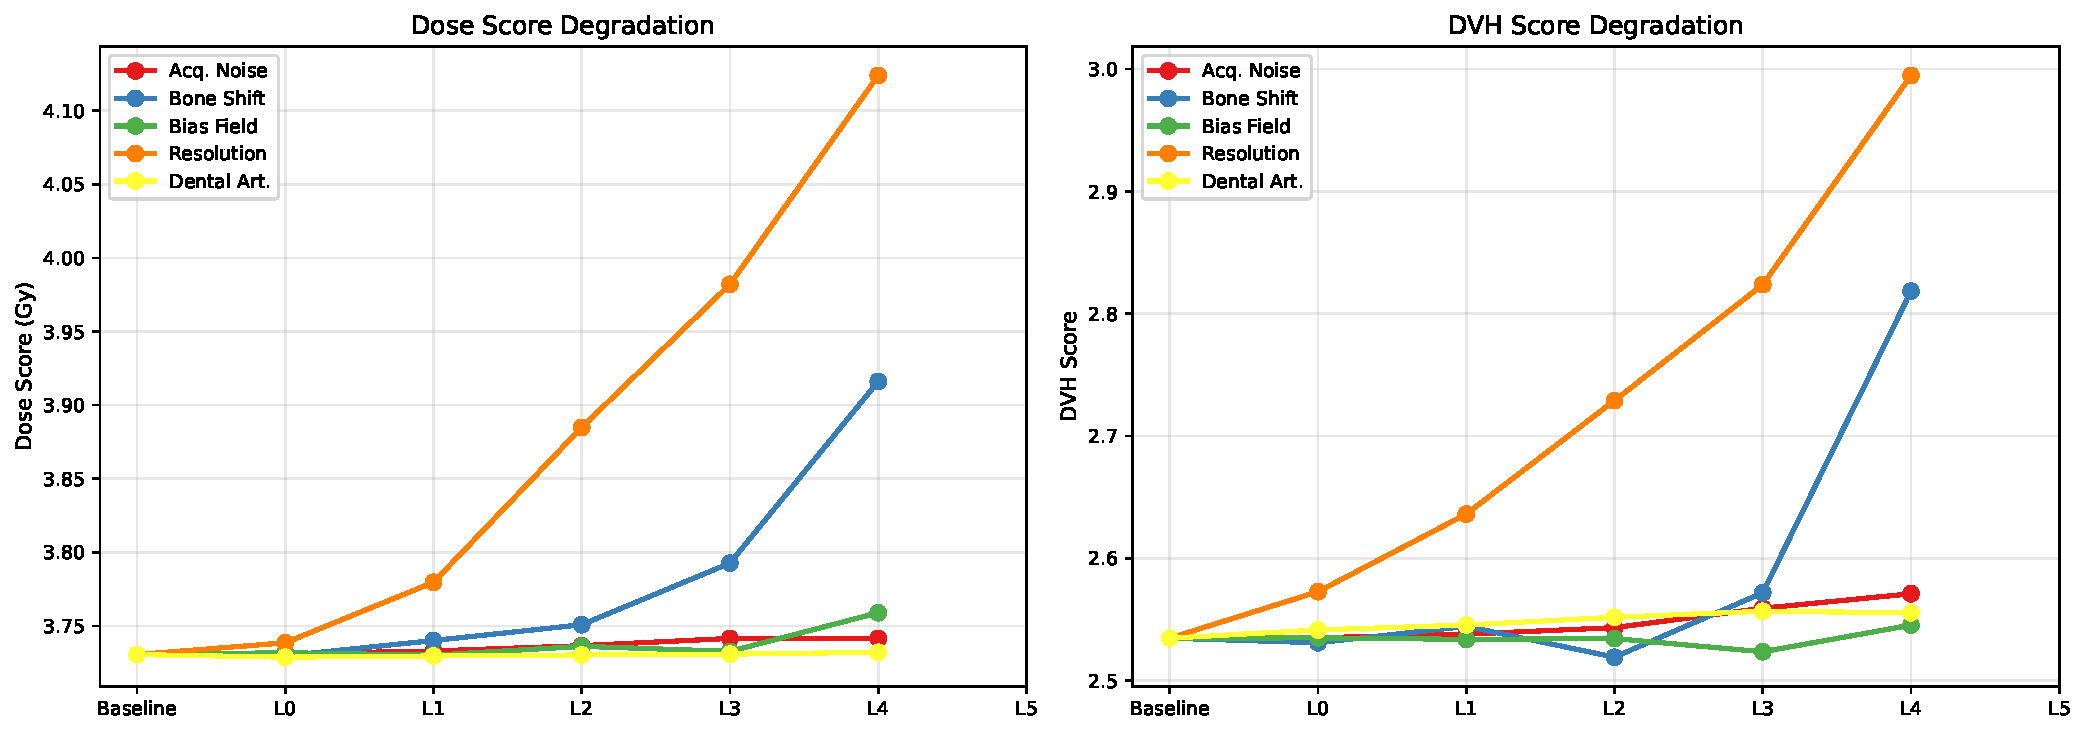
\includegraphics[width=0.95\textwidth]{figures/degradation_curves.pdf}
\caption{Degradation curves showing dose score (left) and DVH score (right) as perturbation severity increases from Baseline through up to 5 levels. P4 (resolution) degrades linearly from the mildest level; P2 (bone shift) shows a late take-off at L4--L5; P1, P3, and P5 remain flat.}
\label{fig:curves}
\end{figure}

\subsection{Degradation Heatmap}

Figure~\ref{fig:heatmap} provides a per-perturbation breakdown of dose and DVH score deltas, highlighting the contrast between P4 and the remaining perturbations.

\begin{figure}[H]
\centering
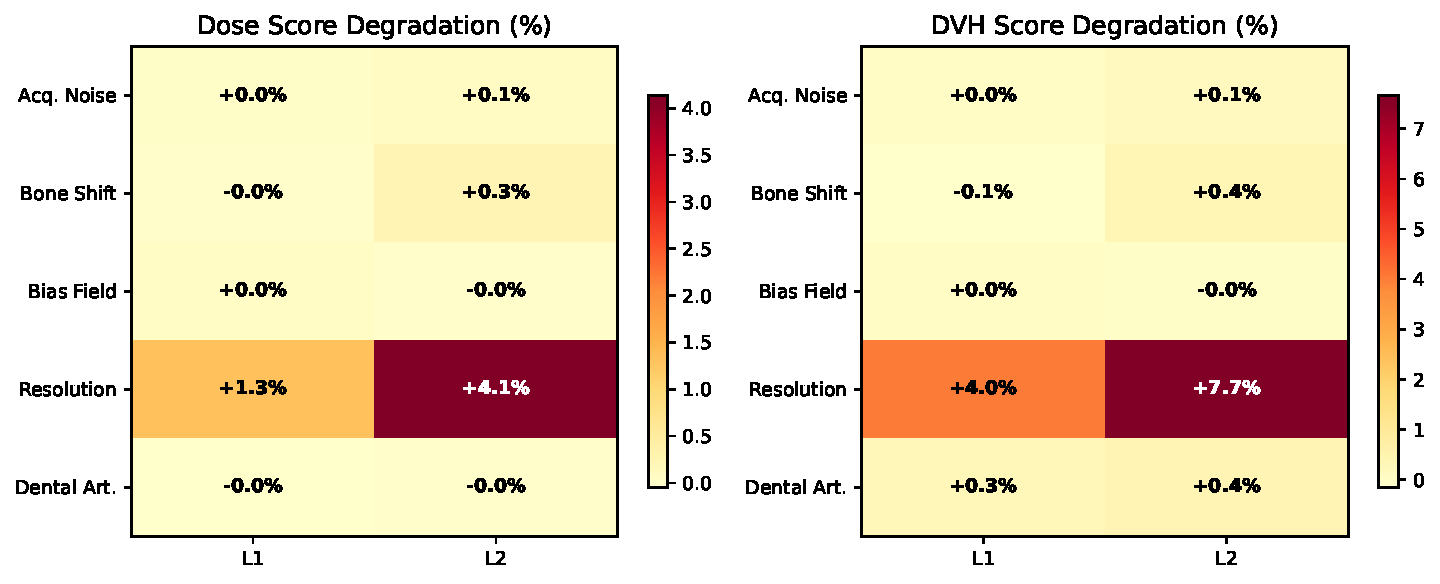
\includegraphics[width=0.85\textwidth]{figures/degradation_heatmap.pdf}
\caption{Heatmap of percentage degradation in dose score and DVH score by perturbation condition. P4 shows progressive degradation from L0 (+1.5\% DVH) to L4 (+18.2\% DVH); P2 shows a late take-off at L5 (+11.2\% DVH). All other cells remain below 1.5\%.}
\label{fig:heatmap}
\end{figure}

\subsection{Per-Structure Analysis}

Figure~\ref{fig:radar} shows the per-structure DVH metric errors under each perturbation. Resolution degradation particularly affects parotid glands, larynx, and mandible---structures with complex geometry where spatial blurring shifts dose-volume boundaries.

\begin{figure}[H]
\centering
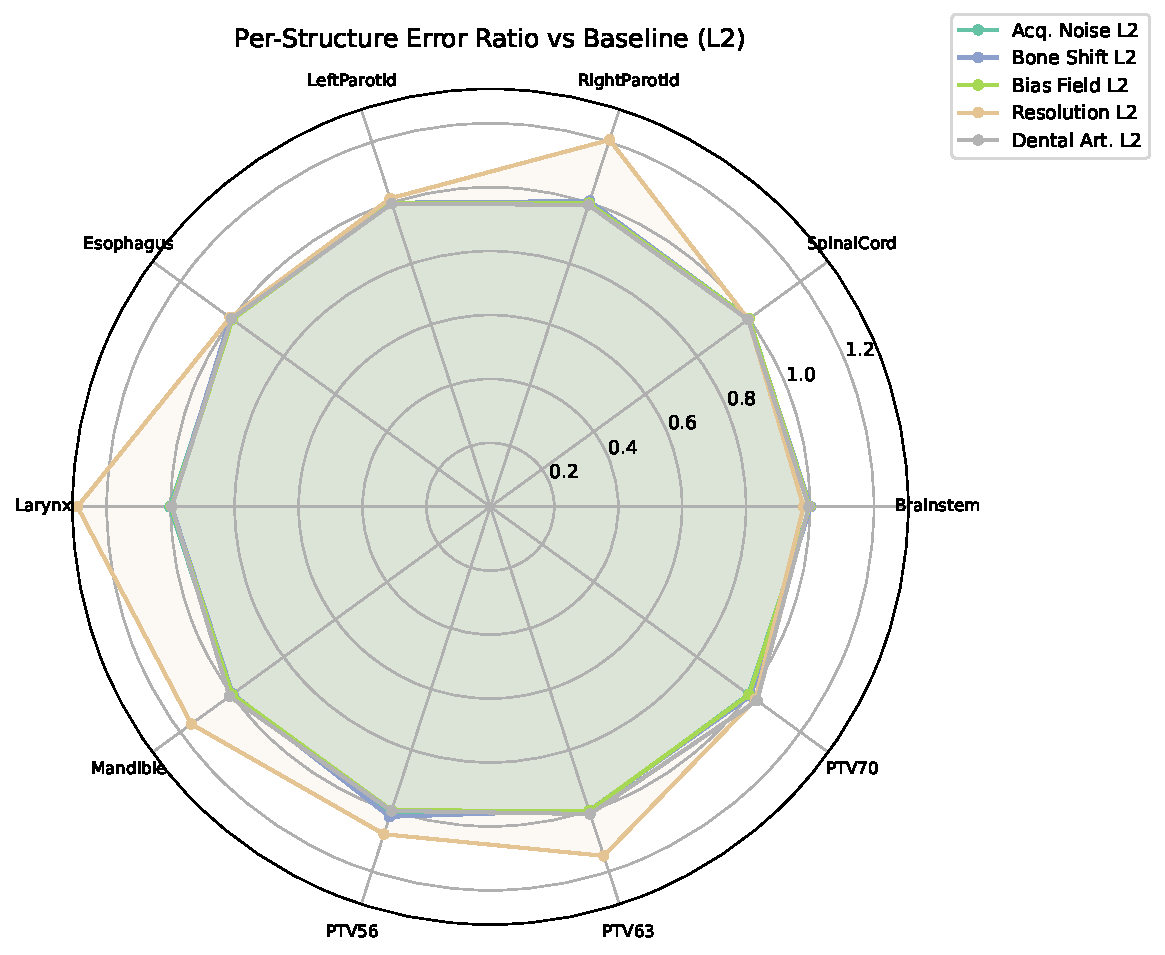
\includegraphics[width=0.85\textwidth]{figures/structure_radar.pdf}
\caption{Radar chart of per-structure DVH errors across perturbation conditions. Baseline is shown as the reference ring; P4/L2 expands outward on structures with dose gradients near boundaries.}
\label{fig:radar}
\end{figure}

\subsection{Visual Examples}

Figures~\ref{fig:ct_slices} and \ref{fig:dose_diff} show representative axial CT slices under each perturbation and the corresponding dose difference maps.

\begin{figure}[H]
\centering
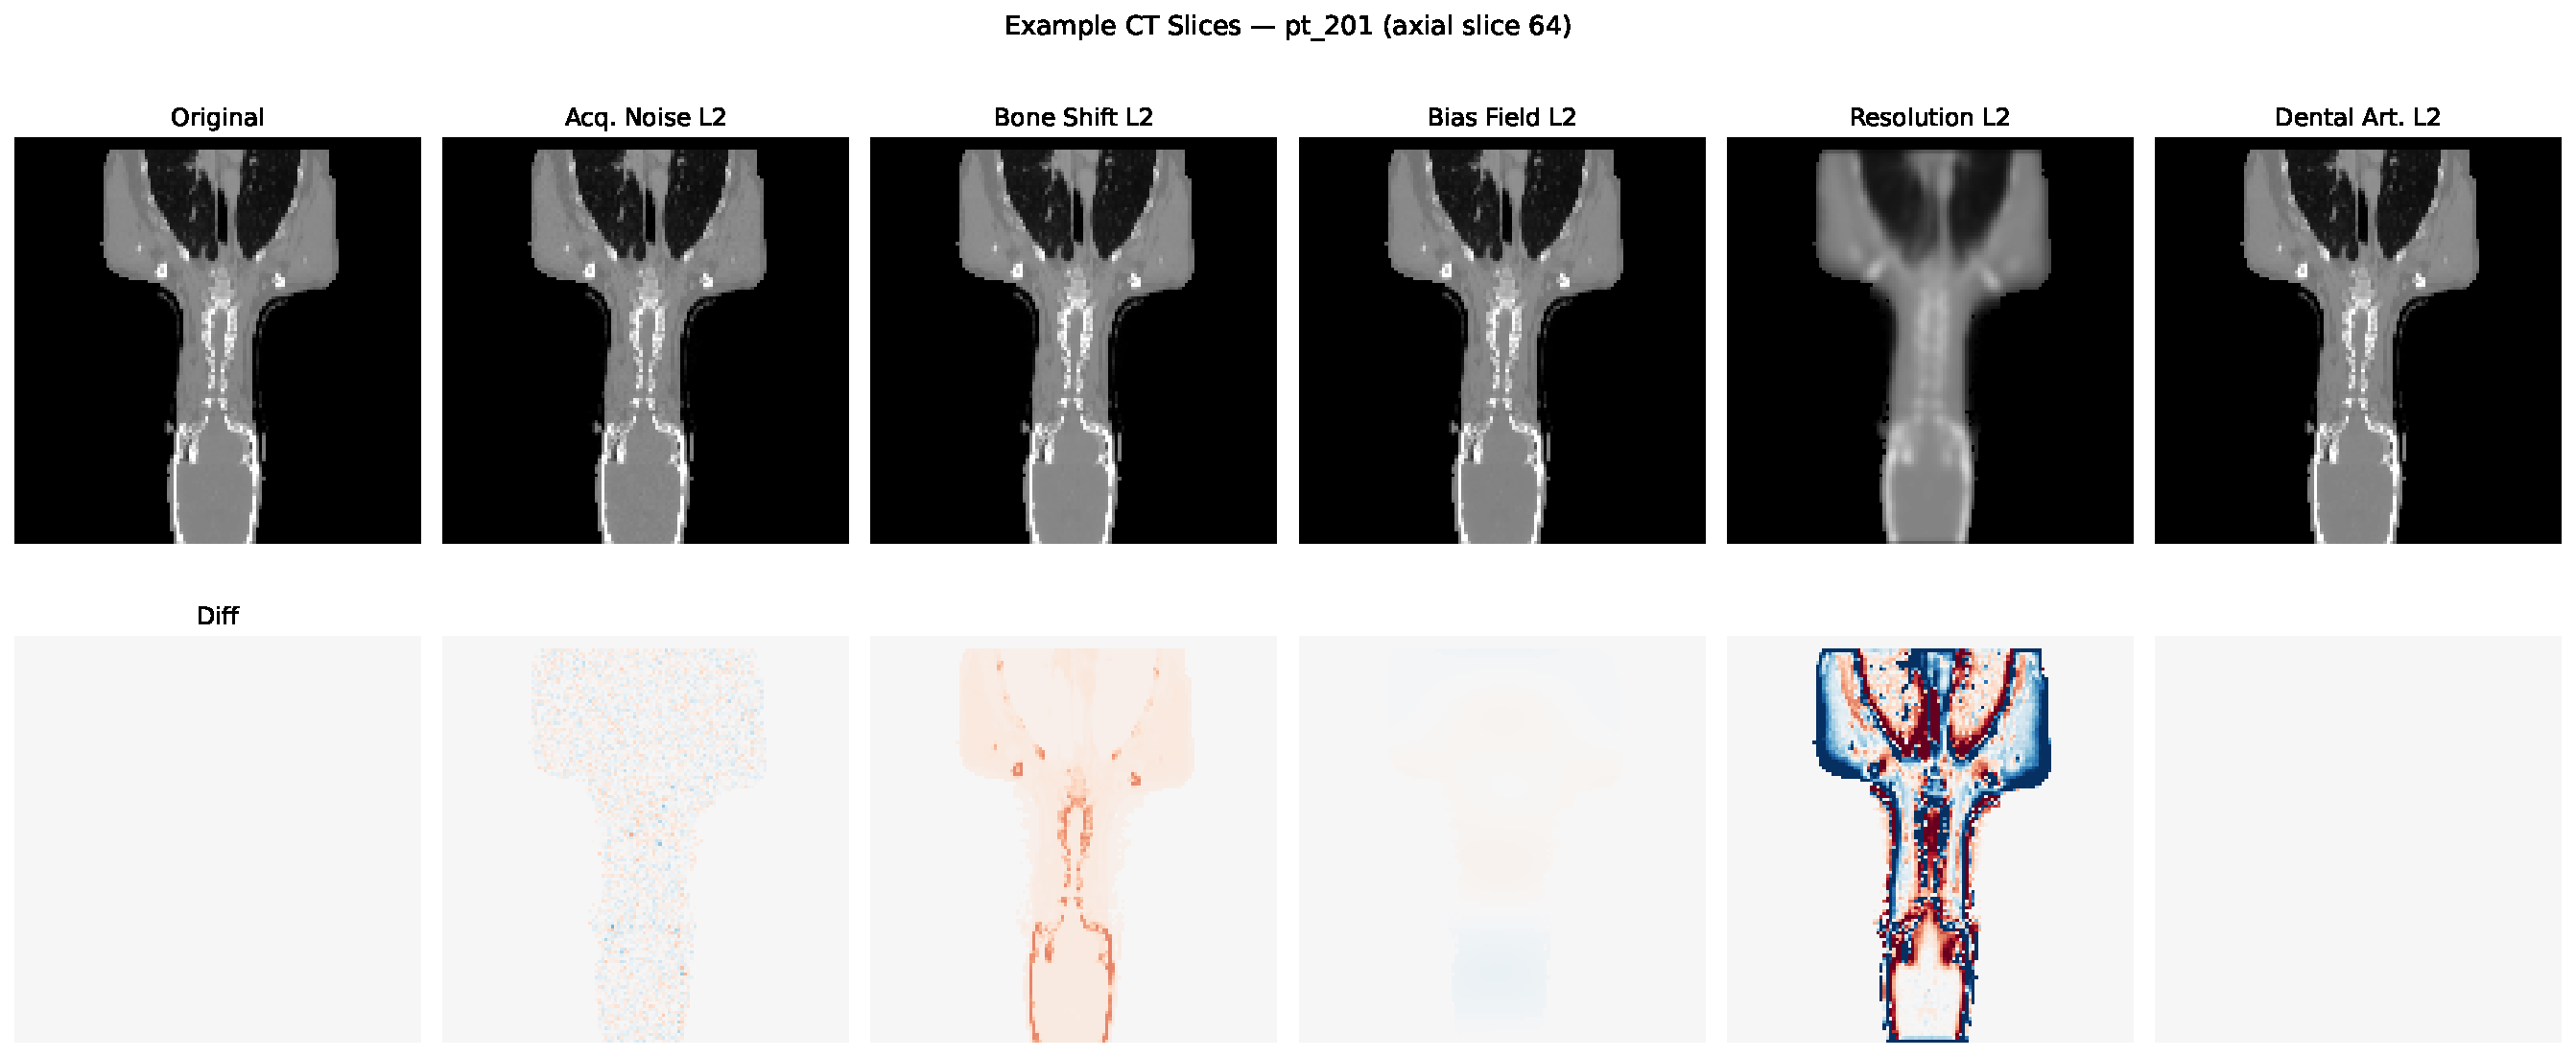
\includegraphics[width=0.95\textwidth]{figures/ct_slices.pdf}
\caption{Axial CT slices (coronal view, head at top) for a representative patient under each perturbation at L2. Top row: perturbed CT; bottom row: difference from original. P1 (noise) and P3 (bias field) produce subtle changes; P2 (bone shift) shows intensity shifts in dense structures; P4 (resolution) visibly blurs tissue boundaries; P5 (dental) adds radial streaks near the mandible.}
\label{fig:ct_slices}
\end{figure}

\begin{figure}[H]
\centering
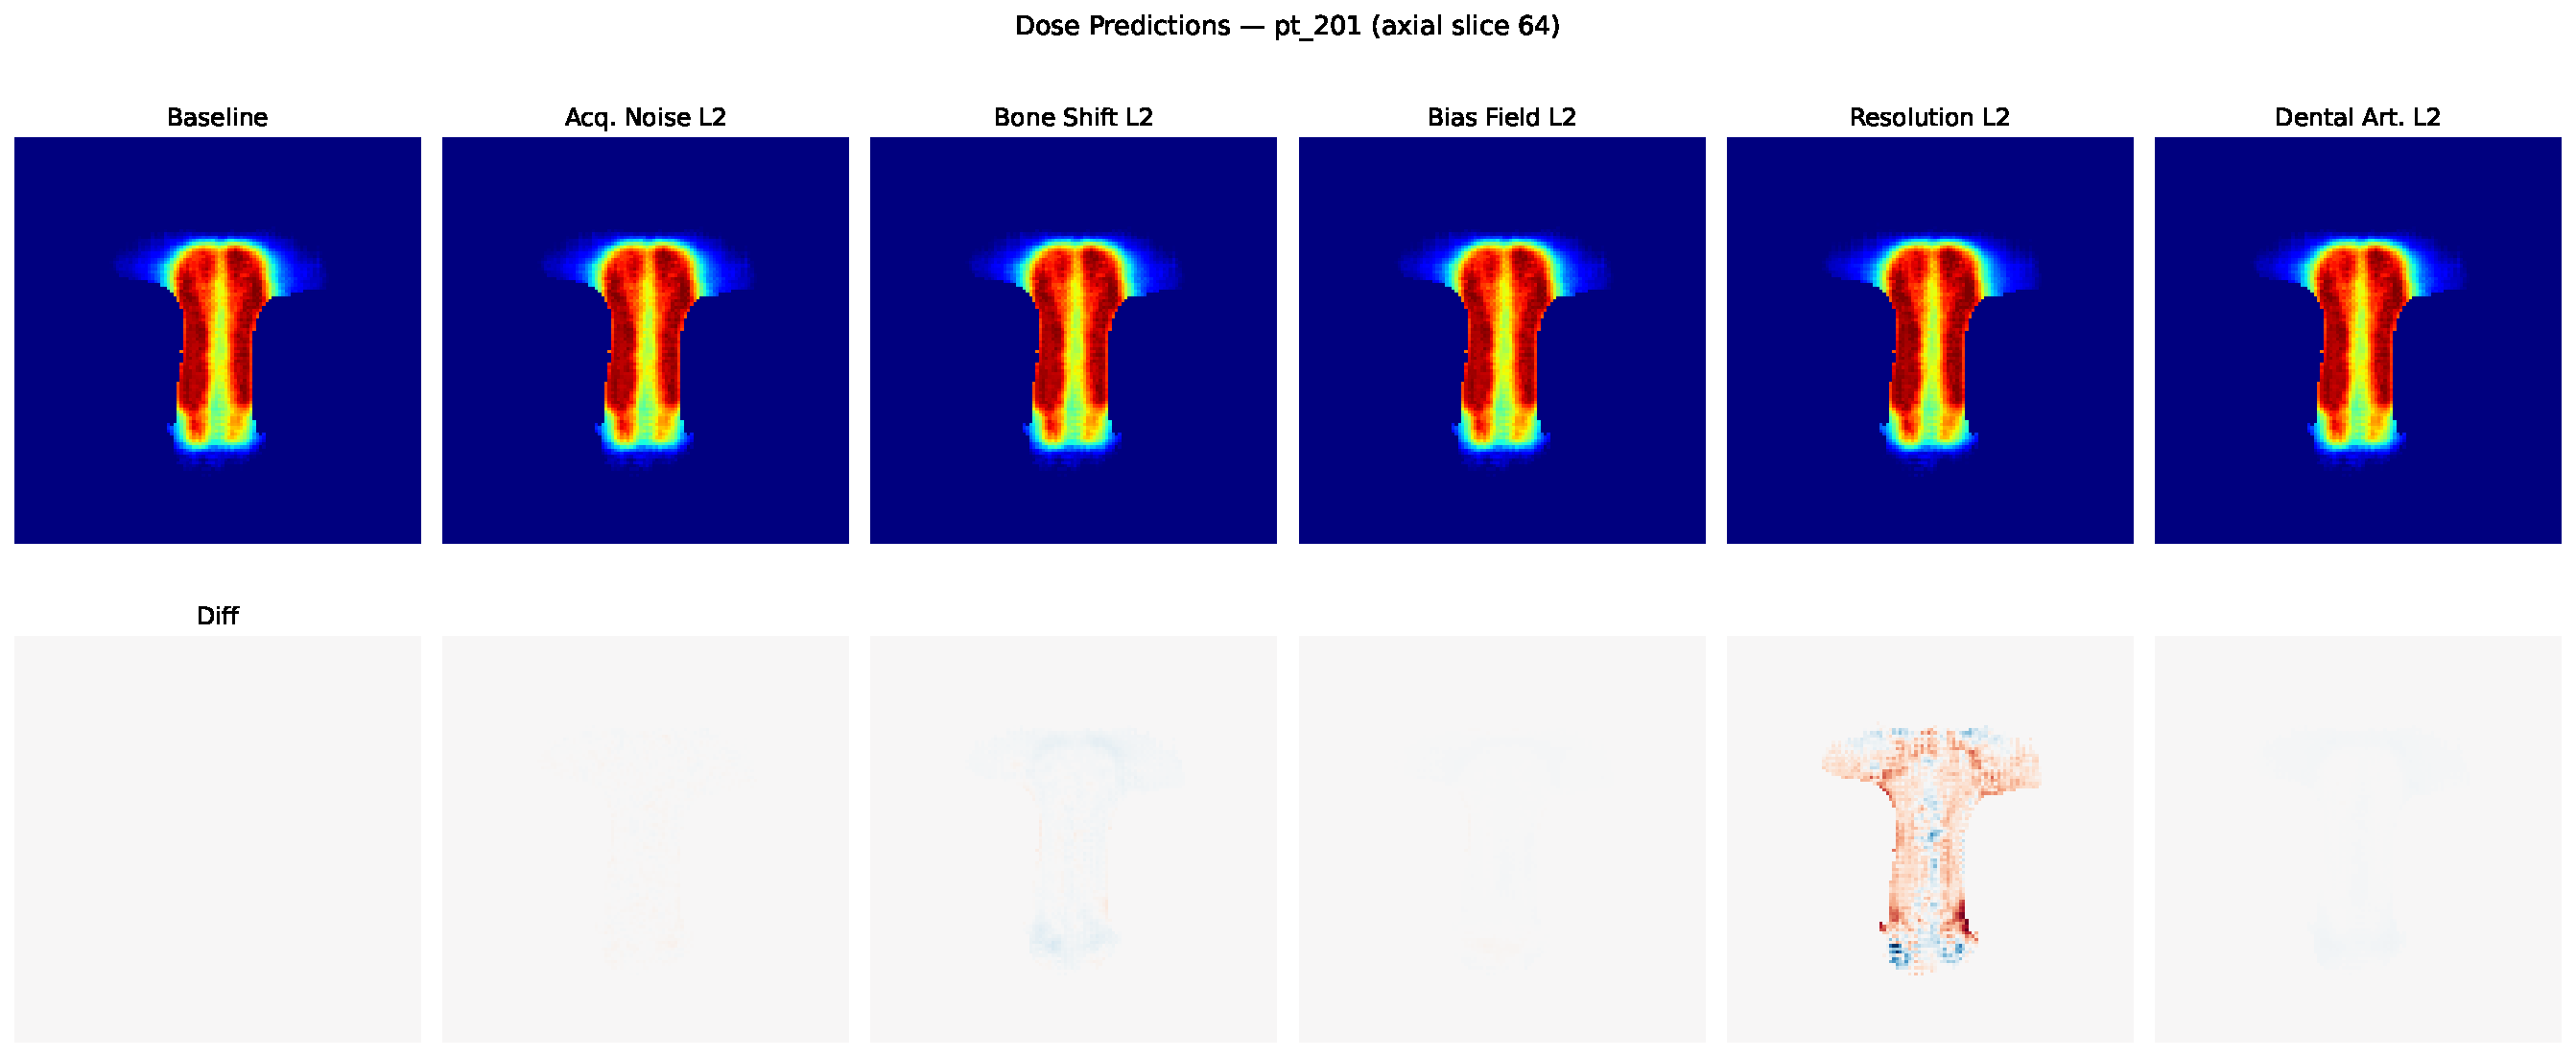
\includegraphics[width=0.95\textwidth]{figures/dose_difference_maps.pdf}
\caption{Dose predictions (top, coronal view) and difference maps (bottom, perturbed $-$ baseline) for the same patient. P4 (resolution) produces spatially structured dose errors concentrated at organ boundaries, consistent with its dominant impact on DVH metrics.}
\label{fig:dose_diff}
\end{figure}

\section{Discussion}

\subsection{Key Findings}

\begin{enumerate}
    \item \textbf{Robust to most intensity-domain perturbations}: P1 (noise), P3 (bias field), and P5 (dental artifacts) cause $\leq$1.4\% DVH degradation even at their highest severity levels (L5), confirming that the model has learned dose-relevant features that are largely invariant to additive noise, smooth intensity fields, and localized metal artifacts.

    \item \textbf{Resolution degradation: immediate, linear sensitivity}: P4 is the dominant perturbation, with DVH degradation beginning at the mildest level tested (L0: $\sigma_z = 0.5$ vox, +1.5\% DVH) and climbing approximately linearly to +18.2\% DVH at L4 ($\sigma_z = 4.0$ vox). There is no safe threshold below which blur is tolerable---even sub-voxel smoothing degrades predictions. Blurring degrades the model's ability to localize organ boundaries, which directly affects DVH metric computation.

    \item \textbf{Bone shift: late threshold effect}: P2 remains flat through L3 ($\Delta_\text{bone} = 250$~HU) but takes off sharply at L4--L5, reaching +11.2\% DVH at L5 ($\Delta_\text{bone} = 1000$~HU). This sudden onset suggests a threshold near $\Delta_\text{bone} \approx 500$~HU, well above typical calibration drift (10--50~HU), indicating the model is safe against realistic calibration errors.

    \item \textbf{DVH more sensitive than dose score}: Resolution degradation causes +4.0\% DVH degradation but only +1.3\% dose score degradation at L1. DVH metrics, which depend on structure-specific dose statistics, are more sensitive to boundary shifts than voxel-wise MAE. This pattern holds across all levels.

    \item \textbf{Structure-dependent vulnerability}: Under P4, parotid glands, larynx, and mandible show the largest DVH increases, likely because these structures have steep dose gradients at their boundaries. Structures in low-gradient regions (e.g., spinal cord) are less affected.
\end{enumerate}

\subsection{Comparison with Adversarial Results (Report~1)}

The contrast between adversarial and physics-based perturbations is striking:

\begin{table}[H]
\centering
\caption{Comparison of adversarial attacks (Report~1) vs.\ physics-based perturbations at similar HU magnitudes.}
\label{tab:comparison}
\begin{tabular}{@{}lccl@{}}
\toprule
\textbf{Perturbation Type} & \textbf{Approx.\ HU} & \textbf{Dose $\Delta$} & \textbf{Nature} \\
\midrule
FGSM, $\epsilon=0.01$ & $\sim$41 HU & +30.4\% & Worst-case gradient direction \\
PGD, $\epsilon=0.01$ & $\sim$41 HU & +21.3\% & Iterative worst-case \\
P1 noise, L5 & $\sigma=$100--160 HU & +0.3\% & Random Gaussian \\
P2 bone shift, L5 & 100--1000 HU & +5.0\% & Systematic calibration \\
P3 bias field, L5 & $\pm$200 HU & +0.8\% & Smooth spatial field \\
\bottomrule
\end{tabular}
\end{table}

Even at extreme perturbation amplitudes (L5: $\sigma = 100$--160~HU for noise, $\Delta = 1000$~HU for bone shift), physically motivated perturbations cause at most +5.0\% dose degradation (P2/L5), compared to +30\% from FGSM at just 41~HU. At comparable HU magnitudes, the gap between adversarial and realistic impacts exceeds 100$\times$. This confirms that the model's adversarial vulnerability (Report~1) does not translate to practical fragility under real imaging conditions---real-world CT variability does not follow adversarial gradient directions.

\subsection{Clinical Implications}

\begin{itemize}
    \item \textbf{CT spatial resolution matters most}: Clinical sites using thicker CT slices or smoother reconstruction kernels should expect degradation in dose prediction accuracy---even sub-voxel blur is detectable. Standardizing spatial resolution across sites would be the single most impactful quality control measure.
    \item \textbf{Intensity variations are well-tolerated}: Scanner noise, bias fields, and dental metal artifacts have negligible impact ($\leq$1.4\% DVH) even at extreme amplitudes, supporting cross-scanner deployment.
    \item \textbf{Calibration drift is safe within clinical ranges}: Bone-weighted HU shifts only become problematic above $\sim$500~HU, far beyond typical inter-scanner calibration drift (10--50~HU). However, sites with severely miscalibrated scanners should be aware of the threshold.
    \item \textbf{No retraining needed for most variations}: The model's inherent robustness to P1, P3, and P5 suggests that data augmentation or adversarial training is unnecessary for handling typical CT intensity variations.
\end{itemize}

\subsection{Limitations}

\begin{itemize}
    \item \textbf{2D perturbation design}: P5 (dental artifact) applies 2D streak patterns extruded along z; real metal artifacts have more complex 3D geometry.
    \item \textbf{Discrete severity levels}: While 4--5 levels per perturbation provide good threshold identification, continuous severity sweeps could reveal finer-grained threshold effects, particularly for P2 between L3 and L5.
    \item \textbf{Single model}: Results are specific to this architecture and training configuration; other models may have different robustness profiles.
    \item \textbf{DVH score limitations}: DVH metrics aggregate information across structures; focal dose errors in small regions may be masked by structure-level averaging.
    \item \textbf{Noise applied per-voxel}: P1 noise is i.i.d.\ per voxel; real CT noise has spatial correlations from reconstruction.
\end{itemize}

\section{Conclusion}

This evaluation demonstrates that the 3D U-Net dose prediction model is highly robust to clinically plausible CT imaging variations. Among five perturbation families spanning the major sources of CT variability:

\begin{enumerate}
    \item \textbf{Three of five} perturbation families (noise, bias field, dental artifacts) cause $\leq$1.4\% DVH degradation even at extreme severity levels (L5), confirming robust invariance to intensity-domain variations.
    \item \textbf{Resolution degradation} is the dominant sensitivity, with no safe threshold---degradation begins at L0 ($\sigma_z = 0.5$ vox, +1.5\% DVH) and reaches +18.2\% DVH at L4 ($\sigma_z = 4.0$ vox), identifying CT spatial resolution as the primary quality control factor.
    \item \textbf{Bone-weighted calibration shift} shows a threshold effect, remaining flat through L3 ($\Delta_\text{bone} = 250$~HU) before taking off at L4--L5 (up to +11.2\% DVH at $\Delta_\text{bone} = 1000$~HU). Typical clinical calibration drift is well below this threshold.
    \item The $>$100$\times$ gap between adversarial and realistic perturbation impacts confirms that the model's adversarial vulnerability (Report~1) does not translate to practical fragility under real imaging conditions.
\end{enumerate}

These findings support the model's suitability for multi-site clinical deployment, provided that CT spatial resolution is standardized or accounted for in the prediction pipeline.

\section{Reproducibility}

\begin{verbatim}
# Step 1: Generate perturbed CT volumes
cd open-kbp-modified/
python openkbp_hn_robustness/generate_perturbed_data.py

# Step 2: Run inference on all conditions (requires GPU + TF 2.18.0)
python openkbp_hn_robustness/run_inference.py

# Step 3: Evaluate metrics (CPU only)
python openkbp_hn_robustness/evaluate_metrics.py

# Step 4: Generate figures
python openkbp_hn_robustness/visualize_results.py
\end{verbatim}

Configuration: \texttt{openkbp\_hn\_robustness/configs/default.yaml}

\section*{Acknowledgments}

This work builds upon the OpenKBP Grand Challenge dataset and baseline implementation. Computation performed on RunPod cloud infrastructure with NVIDIA RTX 3090 GPU.

\end{document}
